\documentclass[12pt,frenchb]{book}

\usepackage[utf8]{inputenc}
\usepackage[T1]{fontenc}
\usepackage{babel}

\usepackage{mathtools,amssymb,tabularx}
\pagestyle{empty}
\usepackage{geometry}
\geometry{margin=1.5cm}
\renewcommand{\thesection}{\Roman{section}.}



\begin{document}
NOM:

NOM:
\chapter{Activité de groupe}
%pour ne pas avoir de numéro de chapitre mettre chapter*

\begin{center}
Activité de gpe
\end{center}
Objectifs :
\parbox[t]{0.8\linewidth}{
\begin{itemize}
\item introduire
\item utiliser
\item créer
\item programmer
\end{itemize}}

\section{A l'aide de geogebra}

Activité 4 p 9 
\begin{enumerate}
\item \dotfill
\item
\begin{enumerate}
\item Lorsque $p=1$. A partir du rang \ldots (c'est-à-dire pr tt $n\geqslant$\ldots), on a $U_{n}\geqslant10^{1}$
\item \dotfill
\item \dotfill
\end{enumerate}
\end{enumerate}
\medskip
Conclusion


\dotfill

\dotfill 

\dotfill

\section{A l'aide d'un tableur}

\begin{minipage}{0.2\linewidth}
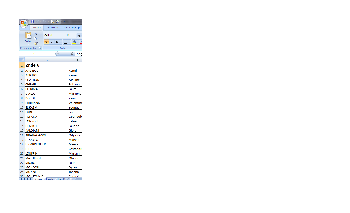
\includegraphics[scale=3]{essaitab.eps}
\end{minipage}\hfill
\begin{minipage}{0.7\linewidth}
\begin{enumerate}
\item Quelle formule entrée ds la cellule B4 et recopiée vers le bas permet de calculer ts les termes de la suite $U_{n}$ ? \par \dotfill
\item A l'aide de l'impression écran ..... $10^{5}\  (p=5)$\par \dotfill \par \dotfill
\item A l'aide de votre... \par \dotfill \par \dotfill 

\textit{Appeler le professeur}

\end{enumerate}
\section{A l'aide de la calculatrice}

Obtenir....

\end{minipage}

\begin{tabularx}{\linewidth}{|>{\centering\bfseries} X|>\centering X|>\centering X|>\centering X|}
\hline
&$p$&$U$&$n$\tabularnewline
\hline
Entrées&2&1&1\tabularnewline
\hline
2eme boucle & & &\tabularnewline
\hline
3eme ligne & & &\tabularnewline
\hline

\end{tabularx}


\end{document}